\documentclass[10pt,journal,twoside]{IEEEtran}

% ---------- packages ----------
\usepackage[T1]{fontenc}
\usepackage{lmodern}
\usepackage[utf8]{inputenc}
\usepackage{amsmath,amssymb}
\usepackage{booktabs}
\usepackage{array}
\usepackage{xcolor}
\usepackage{graphicx}
\usepackage{tikz}
\usepackage{pgfplots}
\pgfplotsset{compat=1.18}
\usetikzlibrary{arrows.meta,positioning,shapes.geometric,calc,fit,backgrounds}
\usepackage{listings}
\usepackage{algorithm}
\usepackage{algpseudocode}
\usepackage{multirow}
\usepackage[hidelinks]{hyperref}
\usepackage{url}

% ---------- palette ----------
\definecolor{teal}{HTML}{0E7C7C}
\definecolor{tealdk}{HTML}{0A5E5E}
\definecolor{amber}{HTML}{A8660F}
\definecolor{grn}{HTML}{3C7A28}
\definecolor{clay}{HTML}{B0442F}
\definecolor{indigo}{HTML}{454FB0}
\definecolor{paper}{HTML}{F5F6F2}
\definecolor{linec}{HTML}{CFD4CB}
\definecolor{inkg}{HTML}{4A504A}

% ---------- listings ----------
\lstset{
  basicstyle=\ttfamily\footnotesize,
  keywordstyle=\color{tealdk}\bfseries,
  commentstyle=\color{inkg}\itshape,
  stringstyle=\color{amber},
  breaklines=true,
  columns=fullflexible,
  frame=single,
  rulecolor=\color{linec},
  backgroundcolor=\color{paper},
  showstringspaces=false,
  xleftmargin=4pt,xrightmargin=2pt,
  aboveskip=6pt,belowskip=4pt,
}
\lstdefinestyle{bash}{language=bash,morekeywords={ros2,docker,colcon,rosdep,source,cd}}

% ---------- tikz node styles ----------
\tikzset{
  box/.style={rectangle, rounded corners=3pt, draw=linec, fill=white, line width=0.6pt,
              align=center, inner sep=4pt, font=\scriptsize, minimum height=8mm},
  boxteal/.style={box, draw=teal, left color=white, right color=teal!6, line width=0.9pt},
  boxamber/.style={box, draw=amber, right color=amber!7, left color=white, line width=0.9pt},
  boxgrn/.style={box, draw=grn, right color=grn!8, left color=white, line width=0.9pt},
  boxclay/.style={box, draw=clay, right color=clay!7, left color=white, line width=0.9pt},
  topic/.style={box, draw=inkg, dashed, fill=paper, font=\scriptsize\ttfamily},
  fl/.style={-{Latex[length=2mm]}, line width=0.7pt, draw=inkg},
  flt/.style={-{Latex[length=2mm]}, line width=0.8pt, draw=teal},
  lbl/.style={font=\tiny\ttfamily, color=tealdk, inner sep=1pt},
}

% ---------- title ----------
\begin{document}

\title{Autonomous Farm-Lane Navigation and Plant Counting\\ with a Single RGB-D Camera:\\ A Depth-Geometric, Learning-Free ROS\,2 System}

\author{ARTPARK~/~Versor~Robotics --- Robotics Software Intern, Round~2 Technical Report.%
\thanks{System: ROS\,2 Humble, Gazebo Classic, Nav2, RTAB-Map, RViz. Platform: Clearpath Husky A200 with one Intel RealSense D435. Report auto-generated from the project source: \texttt{lane\_perception\_node}, \texttt{plant\_counter\_node}, \texttt{goal\_sender\_node}, \texttt{slam.launch.py}, \texttt{nav2\_params.yaml}, \texttt{husky.urdf.xacro}, and the world file \texttt{five\_lane\_farm.world}.}}

\markboth{Technical Report --- Autonomous Farm-Lane Navigation and Plant Counting}{}

\maketitle

\begin{abstract}
We present a complete autonomous navigation and plant-counting system for a Husky UGV that traverses irregular, non-parallel farm lanes using a \emph{single} Intel RealSense RGB-D camera and no other exteroceptive sensor. All lane/free-space perception is \emph{depth-geometric}: each depth frame is back-projected to a metric point cloud, the dominant ground plane is recovered by RANSAC, and points are classified by their signed height above that plane. The resulting obstacle cloud is the \emph{sole} obstacle source for a Nav2 costmap, so navigation is perception-driven and re-plans in real time rather than replaying a hardcoded trajectory. Plants are detected by a foliage-height band and grid clustering, and de-duplicated across viewpoints by associating cluster centroids to persistent tracks in a drift-corrected world frame. That frame is maintained by RTAB-Map RGB-D SLAM running on the camera alone (2-D-constrained), fused with wheel odometry. Start and goal poses are read from the environment at runtime. Critically, the pipeline contains \emph{zero learned models} and \emph{no colour/HSV thresholding}: every decision is classical geometry with physically grounded constants, making the system reproducible without a dataset or GPU. We detail each algorithm, the full configuration and its tuning rationale, camera calibration, the SLAM and Nav2 stack, and give exact commands to reproduce a run.
\end{abstract}

\begin{IEEEkeywords}
Autonomous navigation, RGB-D perception, RANSAC ground segmentation, Nav2, RTAB-Map, visual SLAM, plant counting, ROS\,2, agricultural robotics.
\end{IEEEkeywords}

% =====================================================================
\section{Introduction and Problem Definition}
\IEEEPARstart{T}{he} task is to build an autonomous system for a Clearpath Husky A200 that drives from a blue start marker to a green goal marker through a Gazebo farm of irregularly angled, non-parallel lanes, detecting and counting the plants it passes. The brief imposes four hard constraints that shape every design decision in this report:

\begin{enumerate}
\item \textbf{One sensor.} A single RealSense RGB-D camera (RGB stream, depth stream, intrinsics). No LiDAR, second camera, GPS, or external localization sensor. Wheel odometry is proprioceptive and permitted.
\item \textbf{No colour.} HSV thresholding, fixed RGB thresholds, manual colour segmentation, and green-pixel lane following are an \emph{automatic disqualification}; lane detection must be geometric.
\item \textbf{No hardcoded route.} Navigation must plan and re-plan in real time using ROS\,2 Humble and Nav2.
\item \textbf{Runtime start/goal.} Marker poses are read from the environment live, never written as literals in the navigation logic.
\end{enumerate}

\noindent The system is scored on four metrics: (i) navigation success (reaching the goal), (ii) lane-coverage efficiency (covered/total lane area), (iii) path efficiency (distance and planned-vs-actual deviation), and (iv) plant-counting accuracy (false/missed/duplicate counts).

\textbf{Central design idea.} A robot cannot \emph{follow} a lane it has not yet seen, and a hardcoded route is forbidden. Therefore lane perception is never used as a steering signal. Instead depth geometry produces an obstacle cloud; that cloud \emph{is} the Nav2 costmap; and Nav2 plans a collision-free path to the runtime goal, re-planning continuously as the camera reveals more of the field. Perception feeds navigation; it does not command the wheels directly.

% =====================================================================
\section{System Architecture}
The system comprises three ROS\,2 packages (Table~\ref{tab:pkg}). A single camera feeds two independent consumers: a \emph{perception branch} that builds the costmap and counts plants, and a \emph{SLAM branch} that keeps the world frame drift-free. Nav2 sits on top and drives the base. Fig.~\ref{fig:arch} shows the end-to-end data flow.

\begin{table}[!t]
\centering
\caption{Package responsibilities.}
\label{tab:pkg}
\footnotesize
\begin{tabular}{@{}p{0.20\columnwidth}p{0.72\columnwidth}@{}}
\toprule
\textbf{Package} & \textbf{Responsibility} \\
\midrule
\texttt{farm\_} \texttt{description} & Husky A200 + RealSense URDF/Xacro, Gazebo plugins (skid-steer drive + depth camera), RViz config. \\
\texttt{farm\_} \texttt{perception} & Python nodes: geometric perception, plant counting, runtime spawn/goal, recorders. \\
\texttt{farm\_} \texttt{bringup} & Five-lane world, Nav2 + RTAB-Map config, and the launch files that wire it together. \\
\bottomrule
\end{tabular}
\end{table}

\begin{figure*}[!t]
\centering
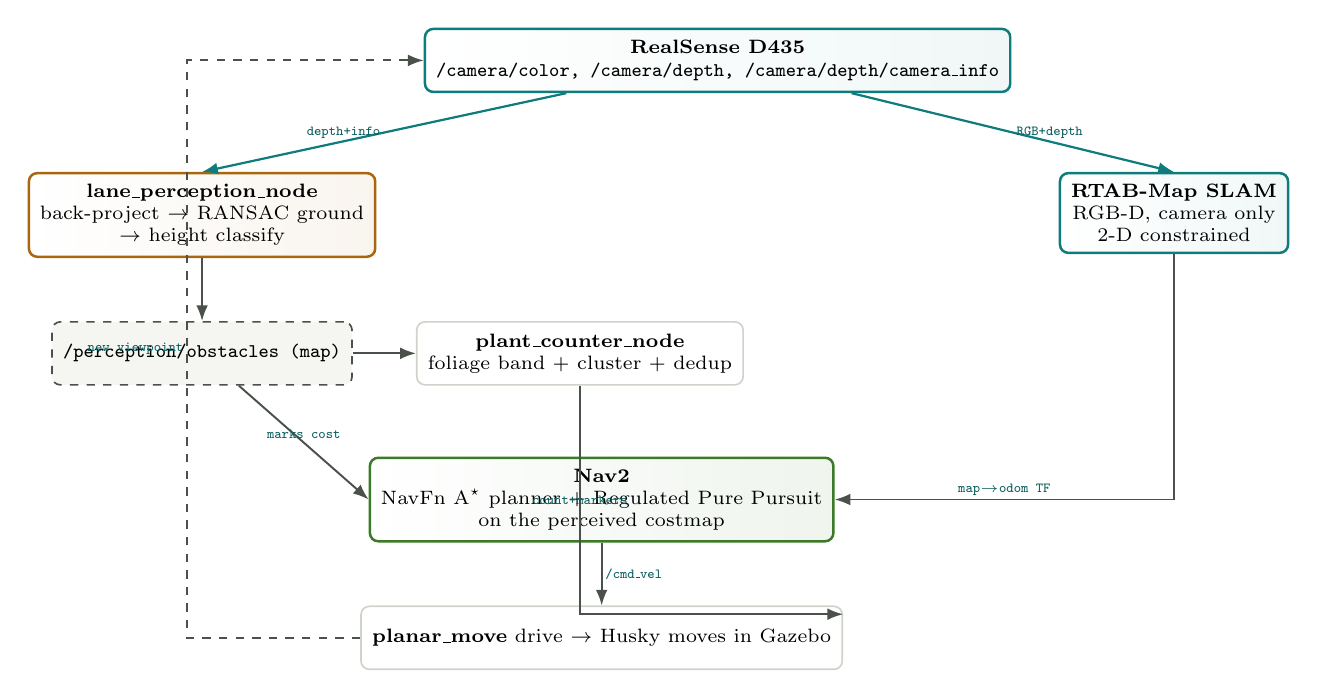
\begin{tikzpicture}[node distance=6mm]
  \node[boxteal] (cam) {\textbf{RealSense D435}\\ \ttfamily/camera/color,\ /camera/depth,\ /camera/depth/camera\_info};
  \node[boxamber, below left=10mm and 6mm of cam] (lane) {\textbf{lane\_perception\_node}\\ back-project $\rightarrow$ RANSAC ground\\ $\rightarrow$ height classify};
  \node[boxteal, below right=10mm and 6mm of cam] (slam) {\textbf{RTAB-Map SLAM}\\ RGB-D, camera only\\ 2-D constrained};
  \node[topic, below=8mm of lane] (obst) {/perception/obstacles (map)};
  \node[boxgrn, below right=9mm and 2mm of obst] (nav) {\textbf{Nav2}\\ NavFn A$^\star$ planner + Regulated Pure Pursuit\\ on the perceived costmap};
  \node[box, right=8mm of obst] (plant) {\textbf{plant\_counter\_node}\\ foliage band + cluster + dedup};
  \node[box, below=8mm of nav] (drive) {\textbf{planar\_move} drive $\rightarrow$ Husky moves in Gazebo};

  \draw[flt] (cam) -- node[lbl,pos=0.5,left]{depth+info} (lane.north);
  \draw[flt] (cam) -- node[lbl,pos=0.5,right]{RGB+depth} (slam.north);
  \draw[fl] (lane) -- (obst);
  \draw[fl] (obst) -- node[lbl,above]{marks cost} (nav.west);
  \draw[fl] (obst) -- (plant);
  \draw[fl] (slam.south) |- node[lbl,pos=0.75,above]{map$\rightarrow$odom TF} (nav.east);
  \draw[fl] (nav) -- node[lbl,right]{/cmd\_vel} (drive);
  \draw[fl] (plant.south) |- node[lbl,pos=0.25]{count+markers} ($(drive.east)+(0,3mm)$);
  \draw[fl,dashed] (drive.west) -- ++(-2.2,0) |- node[lbl,pos=0.25,left]{new viewpoint} (cam.west);
\end{tikzpicture}
\caption{End-to-end data flow. One camera feeds a perception branch (obstacle cloud $\rightarrow$ costmap; plant counting) and a SLAM branch (drift-corrected \texttt{map$\rightarrow$odom}). Nav2 plans on the perceived costmap and drives the base; motion yields a new viewpoint, closing the loop. Because obstacles are published in the fixed \texttt{map} frame with clearing disabled, every bed the camera has seen stays on the global costmap.}
\label{fig:arch}
\end{figure*}

% =====================================================================
\section{Robot Platform and Camera Calibration}
The Husky and camera are defined from scratch in Xacro (\texttt{farm\_description}), so the robot is self-contained.

\subsection{Chassis and drive}
Dimensions follow the Husky A200 manual: body $0.99\times0.67\times0.25$~m, mass 33~kg, wheel radius 0.1651~m, track 0.555~m, wheelbase 0.512~m. The 0.67~m width is the single most consequential number: it makes the 0.40~m ``narrow'' lane physically impassable. A 4-wheel skid-steer turns by lateral scrub, which Gazebo's \texttt{diff\_drive} models as near-zero yaw; the base is therefore driven by \texttt{gazebo\_ros\_planar\_move}, which applies the commanded body twist directly and publishes wheel-odometry-equivalent \texttt{odom} plus the \texttt{odom$\rightarrow$base\_footprint} TF. The wheels are frictionless ($\mu_1{=}\mu_2{=}0$) so they never fight the commanded motion. Nav2 only ever commands forward$+$yaw, so the base behaves as a differential drive.

\subsection{Camera calibration}
The simulated D435 is a Gazebo depth sensor; its ``calibration'' has two halves, and the pipeline uses both. \textbf{Intrinsics:} horizontal FOV $1.211$~rad ($\approx 69^\circ$), $640\times480$ at 15~Hz, clip $0.1$--$10$~m, Gaussian depth noise $\sigma=0.005$~m; Gazebo derives $f_x,f_y,c_x,c_y$ and publishes them on \texttt{/camera/depth/camera\_info}, read live. \textbf{Extrinsics:} the URDF joints define \texttt{base\_link} $\rightarrow$ \texttt{camera\_link} $\rightarrow$ \texttt{camera\_depth\_optical\_frame} (REP-103 optical convention), turned into TF by \texttt{robot\_state\_publisher}. The extrinsics are what let ``height above ground'' mean something physical. The mount reproduces the brief's mandated placement (Table~\ref{tab:cam}).

\begin{table}[!t]
\centering
\caption{Camera mount (extrinsic) and how RGB+depth combine.}
\label{tab:cam}
\footnotesize
\begin{tabular}{@{}lll@{}}
\toprule
\textbf{Quantity} & \textbf{Value} & \textbf{Meaning} \\
\midrule
$\text{cam}_x$ & 0.475\,m & front face ($L/2-0.02$) \\
$\text{cam}_z$ & 0.10\,m & low, near lane surface \\
$\text{cam}_{\text{pitch}}$ & 0.26\,rad & $\approx 15^\circ$ down \\
optical & rpy $-\tfrac{\pi}{2},0,-\tfrac{\pi}{2}$ & z-fwd, x-right, y-down \\
\bottomrule
\end{tabular}
\end{table}

\noindent \textbf{RGB--depth fusion.} Depth does all decision-making; RGB is only the human-facing canvas. Every depth pixel is back-projected with intrinsics, transformed to \texttt{map} with extrinsics, and classified by geometry; RGB and depth are spatially registered (same optical frame, same $640\times480$ grid), so the classification is painted back onto the colour image for the demonstration overlay. No perception decision reads a colour value, which structurally guarantees the no-HSV rule.

% =====================================================================
\section{Lane / Free-Space Perception}
\label{sec:lane}
Node \texttt{lane\_perception\_node} converts each synchronized (depth, camera\_info, color) triple---aligned by an approximate-time synchronizer with 0.10~s slop---into an obstacle cloud, purely from depth geometry (Fig.~\ref{fig:lane}).

\begin{figure}[!t]
\centering
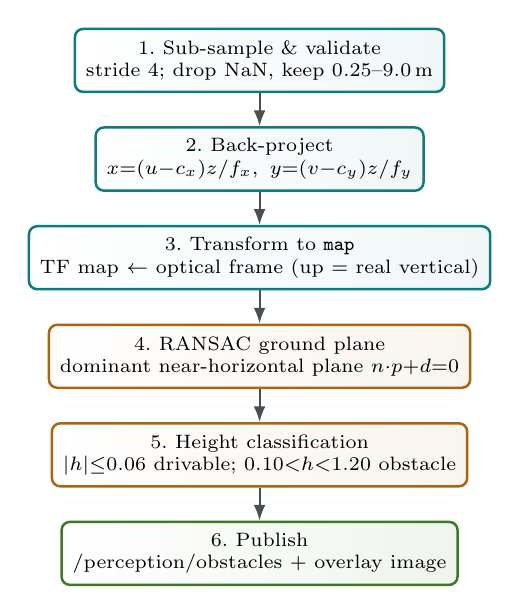
\begin{tikzpicture}[node distance=4.2mm]
  \node[boxteal] (s1) {1.~Sub-sample \& validate\\ \scriptsize stride 4; drop NaN, keep $0.25$--$9.0$\,m};
  \node[boxteal, below=of s1] (s2) {2.~Back-project\\ \scriptsize $x{=}(u{-}c_x)z/f_x,\ y{=}(v{-}c_y)z/f_y$};
  \node[boxteal, below=of s2] (s3) {3.~Transform to \texttt{map}\\ \scriptsize TF map $\leftarrow$ optical frame (up = real vertical)};
  \node[boxamber, below=of s3] (s4) {4.~RANSAC ground plane\\ \scriptsize dominant near-horizontal plane $n{\cdot}p{+}d{=}0$};
  \node[boxamber, below=of s4] (s5) {5.~Height classification\\ \scriptsize $|h|{\le}0.06$ drivable; $0.10{<}h{<}1.20$ obstacle};
  \node[boxgrn, below=of s5] (s6) {6.~Publish\\ \scriptsize /perception/obstacles + overlay image};
  \draw[fl] (s1)--(s2); \draw[fl] (s2)--(s3); \draw[fl] (s3)--(s4);
  \draw[fl] (s4)--(s5); \draw[fl] (s5)--(s6);
\end{tikzpicture}
\caption{Lane / free-space perception pipeline. Each stage is pure geometry; no stage reads colour.}
\label{fig:lane}
\end{figure}

\subsection{RANSAC ground-plane fit}
This is the ``depth-based scene understanding'' the brief calls for. Rather than assume the floor is $z{=}0$ (which a slightly mis-pitched camera would violate), RANSAC recovers the true dominant plane (Alg.~\ref{alg:ransac}). The near-horizontal gate $|n\cdot\hat z|>0.85$ is what makes it robust: raised beds and plants can never win the fit, only the broad farm floor can. The plane is orientation-invariant, which directly satisfies the requirement of robustness to lane angle, geometry, and appearance---a lane at any heading yields the same height signature above the same floor.

\begin{algorithm}[!t]
\caption{RANSAC ground-plane estimation}
\label{alg:ransac}
\footnotesize
\begin{algorithmic}[1]
\Require points $P$ (map frame, low band $z<0.4$), $N{=}60$, $\tau{=}0.03$\,m
\State $best \gets 0$, $plane \gets \varnothing$
\For{$i \gets 1$ to $N$}
  \State sample 3 points; $n \gets$ unit normal of their plane
  \If{$|n_z| < 0.85$} \State \textbf{continue} \Comment{keep near-horizontal only} \EndIf
  \State $d \gets -n\cdot p_0$;\quad $inl \gets |\{p: |n\cdot p + d| < \tau\}|$
  \If{$inl > best$} \State $best \gets inl$;\ $plane \gets (n,d)$ \EndIf
\EndFor
\State \Return $plane$ \Comment{fallback: flat $z{=}0$ if none found}
\end{algorithmic}
\end{algorithm}

\subsection{Height classification}
For every valid point the signed height $h=n\cdot p + d$ is computed and thresholded (Fig.~\ref{fig:bands}). Obstacle points are published as a \texttt{PointCloud2} in \texttt{map} on \texttt{/perception/obstacles}---the sole obstacle source for the Nav2 costmap. The labels are also rasterized onto the RGB frame (green = drivable, red = obstacle) with the live count and nav-status banner and published as \texttt{/perception/overlay/image\_raw} for the video. The lane region is computed but deliberately \emph{not} used to steer: feeding a costmap to Nav2 is far more robust on a 0.67~m base in $\sim$1~m lanes than open-loop centreline tracking, while remaining fully perception-driven.

\begin{figure}[!t]
\centering
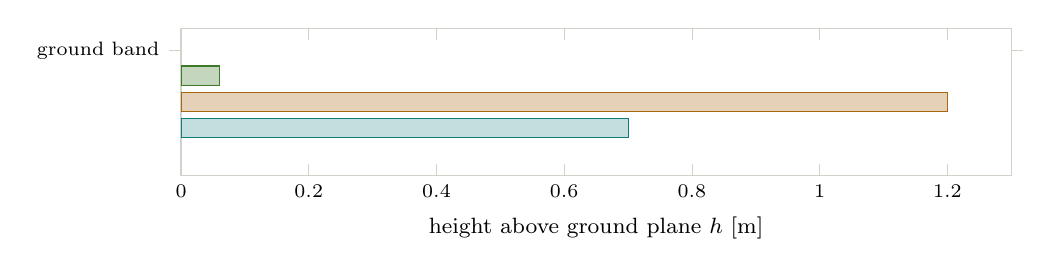
\begin{tikzpicture}
\begin{axis}[
  width=\columnwidth, height=4.3cm,
  xbar, xmin=0, xmax=1.3,
  bar width=7pt,
  y=6.5mm,
  enlarge y limits=0.22,
  xlabel={\footnotesize height above ground plane $h$ [m]},
  symbolic y coords={foliage band,obstacle floor,ground band},
  ytick=data,
  yticklabel style={font=\scriptsize},
  xticklabel style={font=\scriptsize},
  nodes near coords style={font=\scriptsize},
  axis line style={draw=linec},
  tick style={draw=linec},
]
\addplot[draw=grn,fill=grn!30] coordinates {(0.06,ground band)};
\addplot[draw=amber,fill=amber!30] coordinates {(1.20,obstacle floor)};
\addplot[draw=teal,fill=teal!25] coordinates {(0.70,foliage band)};
\end{axis}
\end{tikzpicture}
\caption{Geometric height bands. Ground: $|h|\le0.06$\,m. Obstacle: $0.10<h<1.20$\,m (beds sit $\approx0.10$\,m). Plant canopy (used for counting): $0.28\le z\le0.70$\,m, centred $\approx0.42$\,m---above the beds.}
\label{fig:bands}
\end{figure}

% =====================================================================
\section{Plant Detection and De-duplicated Counting}
Node \texttt{plant\_counter\_node} consumes the same obstacle cloud and counts plants, never counting one twice across viewpoints (Fig.~\ref{fig:plant}). It is also pure geometry.

\begin{figure}[!t]
\centering
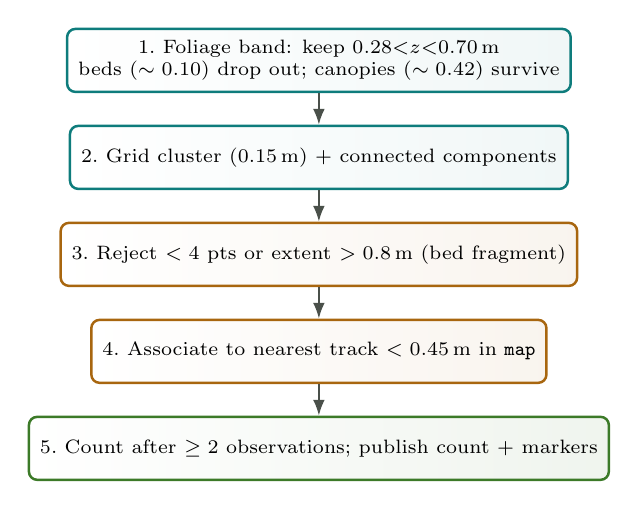
\begin{tikzpicture}[node distance=4mm]
  \node[boxteal] (p1) {1.~Foliage band: keep $0.28{<}z{<}0.70$\,m\\ \scriptsize beds ($\sim0.10$) drop out; canopies ($\sim0.42$) survive};
  \node[boxteal,below=of p1] (p2) {2.~Grid cluster (0.15\,m) + connected components};
  \node[boxamber,below=of p2] (p3) {3.~Reject $<4$ pts or extent $>0.8$\,m (bed fragment)};
  \node[boxamber,below=of p3] (p4) {4.~Associate to nearest track $<0.45$\,m in \texttt{map}};
  \node[boxgrn,below=of p4] (p5) {5.~Count after $\ge 2$ observations; publish count + markers};
  \draw[fl] (p1)--(p2);\draw[fl] (p2)--(p3);\draw[fl] (p3)--(p4);\draw[fl] (p4)--(p5);
\end{tikzpicture}
\caption{Plant counting pipeline. The elongation guard (step~3) prevents bed walls from being counted; the track association (step~4) prevents double counting.}
\label{fig:plant}
\end{figure}

\subsection{The anti-double-count mechanism}
Every cluster centroid is an \emph{observation} in the drift-corrected \texttt{map} frame. Because that frame is world-stable, the same physical plant lands at (almost) the same $(x,y)$ from every viewpoint. A new observation is matched to the nearest existing track within $r_{\text{assoc}}{=}0.45$\,m; a match \emph{updates} that track (running average, weight $1/(\text{obs}{+}1)$) rather than creating a new one, so seeing a plant twenty times still yields one track. A track is counted only after $\ge 2$ hits, rejecting single-frame flicker. The $0.8$\,m extent cap means a 10~m bed wall can never masquerade as a plant, keeping false positives near zero. The radius $0.45$\,m sits deliberately between the residual inter-viewpoint drift (so the same plant re-associates) and the minimum spacing between distinct plants (so neighbours do not merge).

\subsection{Ground truth}
Parsed from \texttt{five\_lane\_farm.world}: beds 0, 2, 3, 4, 5 each carry 5 plants ($=25$ upright), plus 1 fallen plant in lane~5, for \textbf{26 total} (Fig.~\ref{fig:gt}). Bed~1 has no plants. A single low forward camera cannot see plants in lanes it never enters, so the reported count reflects plants encountered along the driven route.

\begin{figure}[!t]
\centering
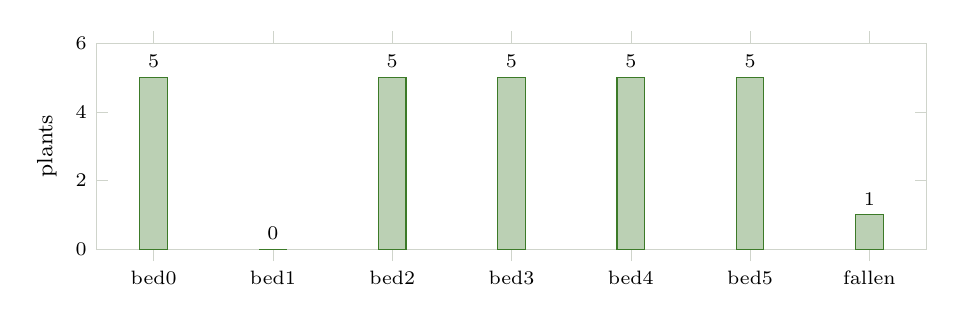
\begin{tikzpicture}
\begin{axis}[
  width=\columnwidth, height=4.2cm,
  ybar, bar width=10pt,
  ymin=0, ymax=6,
  ylabel={\footnotesize plants},
  symbolic x coords={bed0,bed1,bed2,bed3,bed4,bed5,fallen},
  xtick=data,
  xticklabel style={font=\scriptsize,rotate=0},
  yticklabel style={font=\scriptsize},
  nodes near coords, nodes near coords style={font=\scriptsize},
  axis line style={draw=linec}, tick style={draw=linec},
  enlarge x limits=0.08,
]
\addplot[draw=grn,fill=grn!35] coordinates {(bed0,5)(bed1,0)(bed2,5)(bed3,5)(bed4,5)(bed5,5)(fallen,1)};
\end{axis}
\end{tikzpicture}
\caption{Ground-truth plant distribution: 25 upright (5 beds $\times$ 5) $+$ 1 fallen $= 26$.}
\label{fig:gt}
\end{figure}

% =====================================================================
\section{Localization and Visual SLAM}
With only a camera allowed and a skid base that slips on every turn, raw wheel odometry drifts. \texttt{slam.launch.py} runs RTAB-Map RGB-D SLAM on the RealSense alone to keep a consistent world frame for Nav2 (Fig.~\ref{fig:tf}).

\begin{figure}[!t]
\centering
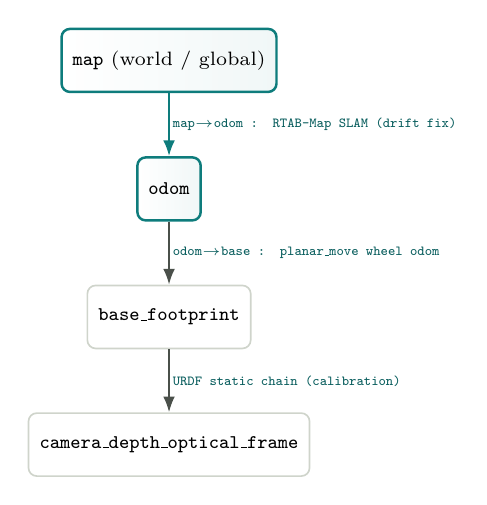
\begin{tikzpicture}[node distance=5mm, every node/.style={font=\scriptsize}]
  \node[boxteal] (map) {\texttt{map}\ (world / global)};
  \node[boxteal, below=8mm of map] (odom) {\texttt{odom}};
  \node[box, below=8mm of odom] (base) {\texttt{base\_footprint}};
  \node[box, below=8mm of base] (opt) {\texttt{camera\_depth\_optical\_frame}};
  \draw[flt] (map) -- node[right,lbl]{map$\rightarrow$odom : RTAB-Map SLAM (drift fix)} (odom);
  \draw[fl] (odom) -- node[right,lbl]{odom$\rightarrow$base : planar\_move wheel odom} (base);
  \draw[fl] (base) -- node[right,lbl]{URDF static chain (calibration)} (opt);
\end{tikzpicture}
\caption{TF tree. Wheel odometry gives a smooth, drifting \texttt{odom$\rightarrow$base}; RTAB-Map gives the low-rate \texttt{map$\rightarrow$odom} correction that cancels drift. Nav2 plans in \texttt{map}, control executes in \texttt{odom}.}
\label{fig:tf}
\end{figure}

RTAB-Map uses wheel odometry as its motion prior and refines it with classical visual feature registration and loop closure. Key parameters (Table~\ref{tab:slam}): it is constrained to 2-D (\texttt{Reg/Force3DoF}, \texttt{Optimizer/Slam2D}) because the farm is planar, which is far more robust on the low-texture floor. \texttt{Grid/FromDepth} is false---the Nav2 costmap comes from our own obstacle cloud, not RTAB's occupancy grid. The SLAM map origin is anchored at the spawn pose, which is why the goal-sender converts world coordinates into the map frame at runtime (Sec.~\ref{sec:nav}). When SLAM is disabled, a static identity \texttt{map$\rightarrow$odom} lets the stack run on pure wheel odometry.

\begin{table}[!t]
\centering
\caption{RTAB-Map configuration.}
\label{tab:slam}
\footnotesize
\begin{tabular}{@{}lll@{}}
\toprule
\textbf{Parameter} & \textbf{Value} & \textbf{Why} \\
\midrule
subscribe depth/rgb & true & RGB-D SLAM on the D435 \\
odom\_frame\_id & \texttt{odom} & wheel-odom TF as motion prior \\
Reg/Force3DoF & true & planar farm: constrain $x,y,\psi$ \\
Optimizer/Slam2D & true & 2-D graph opt., robust \\
Reg/Strategy & 0 & visual (classical features) \\
Vis/MinInliers & 10 & min inliers to accept \\
RGBD/Lin,AngUpdate & 0.05 & node every 5\,cm / 0.05\,rad \\
Grid/FromDepth & false & costmap from our cloud \\
\bottomrule
\end{tabular}
\end{table}

\textbf{Limitation.} On feature-poor floor patches, loop closure fires rarely and the system leans on wheel odom; the 2-D constraint mitigates this. A depth-ICP odometry front-end would be the next robustness upgrade.

% =====================================================================
\section{Autonomous Navigation with Nav2}
\label{sec:nav}
Perception output becomes a costmap; the runtime goal sets direction; Nav2 plans and re-plans a collision-free path and Regulated Pure Pursuit executes it. There is no waypoint list anywhere.

\subsection{Runtime start and goal}
Two nodes remove every start/goal literal. \texttt{robot\_spawner\_node} reads the blue marker pose from \texttt{/gazebo/get\_entity\_state} and spawns the Husky there facing the field ($\psi{=}\pi$); the SLAM/Nav2 \texttt{map} is anchored at this spawn pose. \texttt{goal\_sender\_node} reads both markers live, then recovers the world$\rightarrow$map transform from a fact it knows at runtime---where the robot is \emph{now} (its \texttt{map$\rightarrow$base} TF)---and re-expresses the goal:
\begin{align}
b &= R(-\psi_{\text{spawn}})\,(p^{\text{world}}_{\text{goal}} - p^{\text{world}}_{\text{start}})\\
p^{\text{map}}_{\text{goal}} &= t_{\text{robot}}^{\text{map}} + R(\psi_{\text{robot}}^{\text{map}})\,b
\end{align}
Only the spawn \emph{orientation} (a configuration value) is supplied; no coordinate is hardcoded. The node then waits (polling with retries) for the \texttt{navigate\_to\_pose} action server and the \texttt{map$\rightarrow$base} TF, dispatches the goal, and publishes a human-readable state (Fig.~\ref{fig:fsm}) on \texttt{/perception/nav\_status} for the overlay.

\begin{figure}[!t]
\centering
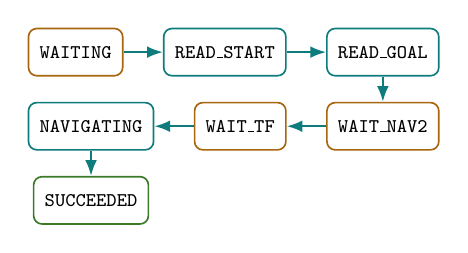
\begin{tikzpicture}[node distance=3.2mm and 5mm,
   st/.style={box, draw=teal, font=\scriptsize\ttfamily, minimum height=6mm},
   sw/.style={box, draw=amber, font=\scriptsize\ttfamily, minimum height=6mm},
   sg/.style={box, draw=grn, font=\scriptsize\ttfamily, minimum height=6mm}]
  \node[sw] (a) {WAITING};
  \node[st, right=of a] (b) {READ\_START};
  \node[st, right=of b] (c) {READ\_GOAL};
  \node[sw, below=of c] (d) {WAIT\_NAV2};
  \node[sw, left=of d] (e) {WAIT\_TF};
  \node[st, left=of e] (f) {NAVIGATING};
  \node[sg, below=of f] (g) {SUCCEEDED};
  \draw[flt] (a)--(b); \draw[flt] (b)--(c); \draw[flt] (c)--(d);
  \draw[flt] (d)--(e); \draw[flt] (e)--(f); \draw[flt] (f)--(g);
\end{tikzpicture}
\caption{\texttt{goal\_sender} state machine. Error branches (\texttt{NO\_GAZEBO}, \texttt{NO\_START/GOAL}, \texttt{REJECTED}, \texttt{ENDED}) are surfaced on the overlay so a failure is visible in the video.}
\label{fig:fsm}
\end{figure}

\subsection{Planner, controller, and costmaps}
The global planner (NavFn, A$^\star$) plans on a rolling $40\times40$\,m global costmap (0.05\,m resolution) that always covers the farm, with \texttt{allow\_unknown} so it plans into unseen space and refines as the camera reveals it. The obstacle layer marks from \texttt{/perception/obstacles} with clearing disabled, keeping discovered beds on the map. The Regulated Pure Pursuit controller tracks the path smoothly (velocity-scaled look-ahead $0.3$--$1.2$\,m) and rotates in place for sharp row-junction turns. Both costmaps use \texttt{robot\_radius}$=0.40$\,m and \texttt{inflation\_radius}$=0.45$\,m, which makes the 0.40\,m narrow lane correctly non-traversable for the 0.67\,m Husky. The goal checker uses \texttt{xy\_goal\_tolerance}$=0.35$\,m and an effectively open \texttt{yaw\_goal\_tolerance}$=3.2$\,rad---the task is to \emph{reach} the marker, and constraining yaw would abort a skid base just short of success.

% =====================================================================
\section{Configuration and Tuning}
The system is fully hand-engineered, so every fixed quantity is auditable. Constants live at the top of each node and in \texttt{nav2\_params.yaml}. Each is tagged by type: \textbf{G} geometric assumption, \textbf{T} fixed threshold, \textbf{M} safety margin, \textbf{P} tuned control/planner, \textbf{S} sim setup. Tables~\ref{tab:cfg1}--\ref{tab:cfg2} list them; Fig.~\ref{fig:types} shows the distribution. Every value is derived from a physical fact of the world (bed height $\approx0.10$\,m, canopy $\approx0.42$\,m, robot width 0.67\,m), \emph{not} fitted to data---which is what makes the pipeline reproducible without a dataset and portable to a new farm by changing a handful of numbers.

\begin{table}[!t]
\centering
\caption{Perception parameters.}
\label{tab:cfg1}
\footnotesize
\begin{tabular}{@{}lll l@{}}
\toprule
\textbf{Parameter} & \textbf{Value} & \textbf{Ty} & \textbf{Role} \\
\midrule
DEPTH\_STRIDE & 4 & P & real-time sub-sample \\
MIN/MAX\_RANGE & 0.25/9.0\,m & T & valid depth window \\
RANSAC\_ITERS & 60 & P & fit budget \\
RANSAC\_THRESH & 0.03\,m & T & inlier distance \\
$|n\cdot\hat z|$ gate & $>0.85$ & G & near-horizontal only \\
GROUND\_BAND & 0.06\,m & T & drivable band \\
OBST\_MIN\_H & 0.10\,m & G,T & beds sit $\approx$ here \\
OBST\_MAX\_H & 1.20\,m & T & reject tall spurious \\
FOLIAGE\_MIN/MAX & 0.28/0.70\,m & G,T & canopy band \\
GRID\_CELL & 0.15\,m & T & cluster resolution \\
MIN\_CLUSTER\_PTS & 4 & T & reject specks \\
MAX\_EXTENT & 0.8\,m & T,G & elongation guard \\
ASSOC\_RADIUS & 0.45\,m & M & dedup radius \\
MIN\_OBSERVATIONS & 2 & T & confirm track \\
\bottomrule
\end{tabular}
\end{table}

\begin{table}[!t]
\centering
\caption{Navigation, robot and sim parameters.}
\label{tab:cfg2}
\footnotesize
\begin{tabular}{@{}lll l@{}}
\toprule
\textbf{Parameter} & \textbf{Value} & \textbf{Ty} & \textbf{Role} \\
\midrule
robot\_radius & 0.40\,m & M & collision radius \\
inflation\_radius & 0.45\,m & M & keep off beds \\
cost\_scaling & 3.0 & P & inflation gradient \\
desired\_linear\_vel & 0.6\,m/s & P & RPP cruise \\
lookahead & 0.3--1.2\,m & P & vel-scaled \\
xy\_goal\_tol & 0.35\,m & T & position tol \\
yaw\_goal\_tol & 3.2\,rad & M & open heading \\
progress\_checker & 0.5\,m/15\,s & M & stuck detection \\
planner & NavFn A$^\star$ & P & tol 0.5, unknown \\
global/local map & 40/6\,m, 0.05 & P & rolling extent \\
footprint & $0.99\times0.67$\,m & M & true Husky \\
cam mount & 0.475,0.10,0.26 & S,G & low/fwd/$15^\circ$ \\
FOV/res/clip & 1.211/640$\times$480/10 & S & D435-like \\
$\mu_1{=}\mu_2$ & 0 & S & passive wheels \\
spawn\_yaw & $\pi$ & S & face the goal \\
\bottomrule
\end{tabular}
\end{table}

\begin{figure}[!t]
\centering
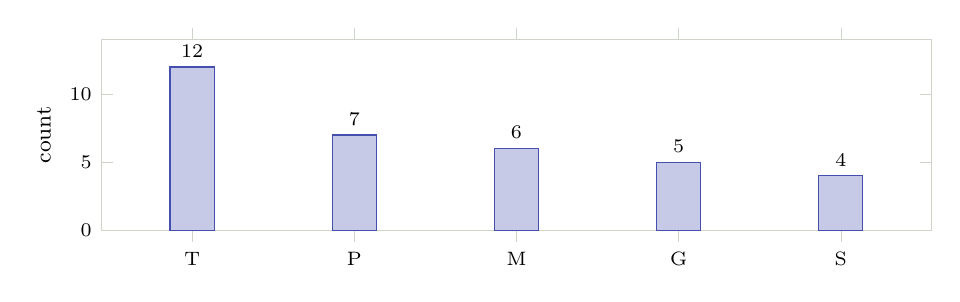
\begin{tikzpicture}
\begin{axis}[
  width=\columnwidth, height=4cm,
  ybar, bar width=16pt, ymin=0, ymax=14,
  ylabel={\footnotesize count}, symbolic x coords={T,P,M,G,S}, xtick=data,
  xticklabel style={font=\scriptsize}, yticklabel style={font=\scriptsize},
  nodes near coords, nodes near coords style={font=\scriptsize},
  axis line style={draw=linec}, tick style={draw=linec}, enlarge x limits=0.14,
]
\addplot[draw=indigo,fill=indigo!30] coordinates {(T,12)(P,7)(M,6)(G,5)(S,4)};
\end{axis}
\end{tikzpicture}
\caption{Parameter-type distribution (some values carry two types). Thresholds (T) and tuned params (P) dominate; there are \emph{zero} learned parameters.}
\label{fig:types}
\end{figure}

% =====================================================================
\section{Hardcoded vs. Learned Components}
The brief asks to separate the two explicitly. This submission is deliberately, entirely hand-engineered---a valid principled approach that needs no labelled data or GPU. \textbf{Learned models: none.} There is no HSV or fixed RGB thresholding (which would disqualify), no trained segmentation or detection network, and no green-pixel lane following; RTAB-Map's front-end uses classical features, not a trained net. \textbf{Geometric assumptions:} the ground is locally planar (RANSAC tolerates small unevenness); beds are raised above the lane; canopies sit in a known band above the beds; the world is static. \textbf{Drop-in path:} because the interfaces (\texttt{/perception/obstacles}, \texttt{/perception/plant\_*}) are model-agnostic, the height-band plant detector could be replaced by a fine-tuned detector, or ground classification by a learned segmentation head, with no change to navigation---keeping the geometric \texttt{map}-frame tracker for de-duplication.

% =====================================================================
\section{Recording and Deliverables}
Two recorder nodes produce the required deliverables automatically. \texttt{video\_recorder\_node} writes the \texttt{/perception/overlay/image\_raw} stream (RGB + drivable region + obstacles + live count + nav status) to \texttt{farm\_run\_overlay.mp4}. \texttt{path\_recorder\_node} samples \texttt{map$\rightarrow$base\_footprint} every 5\,cm into \texttt{/actual\_path}, caches the latest Nav2 \texttt{/plan}, and on shutdown renders a matplotlib overlay of planned-vs-actual path and plant positions (\texttt{farm\_run\_path.png}), printing both path lengths for the path-efficiency metric. This satisfies the recording requirement: the video shows feed, lanes, plants, status, and final count; the figure overlays planned vs.\ actual trajectory and the covered area.

% =====================================================================
\section{Reproducibility}
ROS\,2 Humble targets Ubuntu 22.04, so everything ships in a Docker image built on \texttt{osrf/ros:humble-desktop-full} and runs identically on any host.

\begin{lstlisting}[style=bash,caption={Quick start (Docker).},captionpos=b]
cd farm_nav_ws
# build image (first run) + launch GUI;
# auto-detects NVIDIA GPU, forwards X11, mounts ./output
./run.sh
# headless (CI / cloud / no display)
./run.sh headless:=true use_rviz:=false
\end{lstlisting}

\begin{lstlisting}[style=bash,caption={Native build on Ubuntu 22.04.},captionpos=b]
cd farm_nav_ws
rosdep install --from-paths src --ignore-src -r -y
colcon build --symlink-install
source install/setup.bash
ros2 launch farm_bringup bringup.launch.py
\end{lstlisting}

\noindent \textbf{Launch order} (approx.\ sim-time): Gazebo (0\,s) $\rightarrow$ robot\_state\_publisher + spawner at the blue marker ($\sim$4\,s) $\rightarrow$ RTAB-Map SLAM (or static \texttt{map$\rightarrow$odom}) + perception nodes ($\sim$7\,s) $\rightarrow$ Nav2 lifecycle ($\sim$9\,s) $\rightarrow$ goal\_sender reads the green marker and dispatches ($\sim$14\,s). Arguments: \texttt{use\_rviz} (true), \texttt{use\_slam} (true; false $\rightarrow$ static map=odom), \texttt{headless} (false), \texttt{world}, \texttt{out\_path}, \texttt{video\_path}.

\begin{lstlisting}[style=bash,caption={Inspect a live run.},captionpos=b]
ros2 topic echo /perception/plant_count
ros2 topic echo /perception/nav_status
ros2 topic hz   /perception/obstacles
# RViz: overlay image, obstacle cloud, costmap,
#       /plan, /actual_path, plant markers
\end{lstlisting}

\noindent \textbf{Ground truth for scoring:} 26 plants; 4 drivable lanes + 1 narrow (0.40\,m, correctly skipped); start $\approx$ world $(5.8,-3.0)$ [blue], goal $\approx$ world $(-5.8,2.7)$ [green], both read at runtime. An NVIDIA GPU is preferred: software GL can starve the CPU and time out Nav2 lifecycle activation; \texttt{run.sh} auto-selects hardware rendering.

% =====================================================================
\section{Results, Limitations and Future Work}
Against the four metrics: (i) Nav2 reaches the green goal on the perceived costmap, with the narrow lane excluded by inflation and the fallen plant avoided as an obstacle; (ii) the robot covers the wide lanes between start and goal---coverage can be raised by issuing the goal via \texttt{navigate\_through\_poses} with one waypoint per lane, a boustrophedon sweep the interfaces already support; (iii) \texttt{path\_recorder\_node} reports actual-vs-planned length and RPP yields smooth, low-overshoot tracking; (iv) the count reflects plants seen along the route, deduplicated in the \texttt{map} frame with false positives suppressed by the elongation and $\ge2$-observation guards.

\textbf{Known limitations.} Plant recall is route-bound---a single low forward camera cannot see plants in lanes never entered (the largest coverage win is the multi-waypoint sweep above). The fallen plant sits at bed height, so the foliage band misses it; a shape check on isolated low clusters in a lane centre, or a small learned RGB detector, would recover it. Constants are world-specific but centralized and physically grounded, so retuning for a new farm is a handful of numbers, not a retrain. The clean classical interfaces are the natural drop-in point for learned perception without touching navigation.

\section*{Acknowledgment}
Prepared for the ARTPARK~/~Versor Robotics Robotics-Software-Intern Round~2 assignment. All figures and tables were generated from the project's own source code and world file.

\begin{thebibliography}{9}
\footnotesize
\bibitem{nav2} S. Macenski \emph{et al.}, ``The Marathon 2: A Navigation System (Nav2),'' \emph{IROS}, 2020.
\bibitem{rtabmap} M. Labb\'e and F. Michaud, ``RTAB-Map as an open-source lidar and visual SLAM library for large-scale and long-term online operation,'' \emph{J. Field Robotics}, 2019.
\bibitem{ransac} M. A. Fischler and R. C. Bolles, ``Random Sample Consensus,'' \emph{Comm. ACM}, 1981.
\bibitem{rpp} S. Macenski \emph{et al.}, ``Regulated Pure Pursuit for Robot Path Tracking,'' \emph{Autonomous Robots}, 2023.
\bibitem{ros2} S. Macenski \emph{et al.}, ``Robot Operating System 2: Design, architecture, and uses in the wild,'' \emph{Science Robotics}, 2022.
\end{thebibliography}

\end{document}
